
\documentclass[final]{beamer}



\usepackage[scale=0.8,size=a1]{beamerposter} % Use the beamerposter package for laying out the poster

\usetheme{confposter} % Use the confposter theme supplied with this template
\usepackage{multicol}
\setbeamercolor{block title}{fg=dblue,bg=white} % Colors of the block titles
\setbeamercolor{block body}{fg=black,bg=white} % Colors of the body of blocks
\setbeamercolor{block alerted title}{fg=white,bg=dblue!70} % Colors of the highlighted block titles
\setbeamercolor{block alerted body}{fg=black,bg=dblue!10} % Colors of the body of highlighted blocks
% Many more colors are available for use in beamerthemeconfposter.sty

%-----------------------------------------------------------
% Define the column widths and overall poster size
% To set effective sepwid, onecolwid and twocolwid values, first choose how many columns you want and how much separation you want between columns
% In this template, the separation width chosen is 0.024 of the paper width and a 4-column layout
% onecolwid should therefore be (1-(# of columns+1)*sepwid)/# of columns e.g. (1-(4+1)*0.024)/4 = 0.22
% Set twocolwid to be (2*onecolwid)+sepwid = 0.464
% Set threecolwid to be (3*onecolwid)+2*sepwid = 0.708
%%%%% XAVI %%%%%%%%%%%%%
\newcommand{\memo}[2]{\textcolor{#1}{#2}}
\newcommand{\xavi}[1]{\memo{orange}{#1\\}}

\newlength{\sepwid}
\newlength{\onecolwid}
\newlength{\twocolwid}
\newlength{\threecolwid}
\setlength{\paperwidth}{33.1in} % A0 width: 46.8in
\setlength{\paperheight}{23.4in} % A0 height: 33.1in
\setlength{\sepwid}{0.0\paperwidth} % Separation width (white space) between columns
\setlength{\onecolwid}{0.22\paperwidth} % Width of one column
\setlength{\twocolwid}{0.464\paperwidth} % Width of two columns
\setlength{\threecolwid}{0.708\paperwidth} % Width of three columns
\setlength{\topmargin}{-0.5in} % Reduce the top margin size
%-----------------------------------------------------------

\usepackage{graphicx}  % Required for including images

\usepackage{booktabs} % Top and bottom rules for tables
\usepackage{standalone} % to load standalone file (itkz picture for ex)
\usepackage{array} %finest gestion of tabular
\usepackage{algorithm,algorithmicx,algpseudocode}
\usepackage{setspace}

%----------------------------------------------------------------------------------------
%	TITLE SECTION 
%----------------------------------------------------------------------------------------

%\title{Exploring the dynamic of cultural changes: A model to understand the amphorae production patterns in the Roman Empire} % Poster title
%\title{New perspective on the study of variations in Amphorae production during the Roman Empire} % Poster title
\title{Social learning of pottery-making techniques\\{\huge An Agent Based Model to understand the amphorae production patterns in the Roman Empire}}


\author{Maria Coto- Sarmiento$^{1,2}$, Simon Carrignon$^{1,3}$ and Xavier Rubio-Campillo$^{1}$} % Author(s)

\institute{$^1$Barcelona Supercomputing Center -- $^2$University of Barcelona -- $^3$Universitat Pompeu Fabra} % Institution(s)

%----------------------------------------------------------------------------------------

\begin{document}

\addtobeamertemplate{block end}{}{\vspace*{2ex}} % White space under blocks
\addtobeamertemplate{block alerted end}{}{\vspace*{2ex}} % White space under highlighted (alert) blocks

\setlength{\belowcaptionskip}{2ex} % White space under figures
\setlength\belowdisplayshortskip{2ex} % White space under equations

\begin{frame}[t] % The whole poster is enclosed in one beamer frame

\vspace{-1cm}

\begin{columns}[t] % The whole poster consists of three major columns, the second of which is split into two columns twice - the [t] option aligns each column's content to the top

\begin{column}{\sepwid}\end{column} % Empty spacer column

\begin{column}{\onecolwid} % The first column


\begin{block}{Introduction}

\justify

Our study aims to explore the changes in the large-scale amphorae production within Roman Empire. This study explores the question of transmission on the learning techniques processes. Specifically, we are interested on understanding if pottery-making techniques were transmitted through vertical or horizontal social learning. If vertical transmission predominates in this process then amphorae made in nearby workshops may share more similar traits than amphorae from farthest workshops. We also analysed the correlation between spatial distance and morphometric variation by observing test. In this work we have explored the social learning processes associated with amphorae production through a combination of empirical analysis and theoretical exploration.   

%Material culture variability allows us to interpret the change in the production processes~\cite{lycett}. In particular, this study is exploring this question by analyzing large-scale amphorae production during the Roman Empire. Specifically, we are interested on understanding if pottery-making techniques were transmitted thought vertical or horizontal social learning. If vertical is the one in use, amphorae made in nearby workshops might share more similar traits than amphorae made from farthest workshops, following isolation-by distance~\cite{bjo}.  We test it by observing the existence of a correlation between spatial distance and morphometric variation. In this work we have explored the social learning processes associated with amphorae production through a combination of empirical analysis and theoretical exploration. 

\end{block}

\vspace{-0.5cm}

\begin{block}{Materials}

\justify
We have analyzed 470 amphorae (fig.\ref{fig:betica}~(b)) from 5 different workshops located in \emph{Baetica} (fig.\ref{fig:betica}~(a)). This province supplied a massive quantity of olive oil to the rest of the Empire from the Ist to the IIIrd centuries, and for this reason a large-scale infrastructure of amphorae production was developed here. The same amphoric type (Dressel 20) was produced in several workshops located along the course of the Guadalquivir river. A sample of 90 amphorae was chosen for each of the four analysed workshops. Eight different measures were taken for each amphorae, most of them focused on the rim as an indicator of variability. 


%The workshops were selected from different sites of \emph{Baetica} province in order to know if morphometric distance was correlated with spatial distance\xavi{you can remove this sentence, you already said that they are from Baetica, and that the aim of the study is to see if variation is correlated with distance. A better phrasing:The same amphoric type (Dressel 20) was produced in several workshops located along the course of the Guadalquivir river}
%\xavi{A sample is the entire set of amphorae, not each amphora, so you can't say "90 sample".}

\begin{figure}
\begin{tabular}{cc}


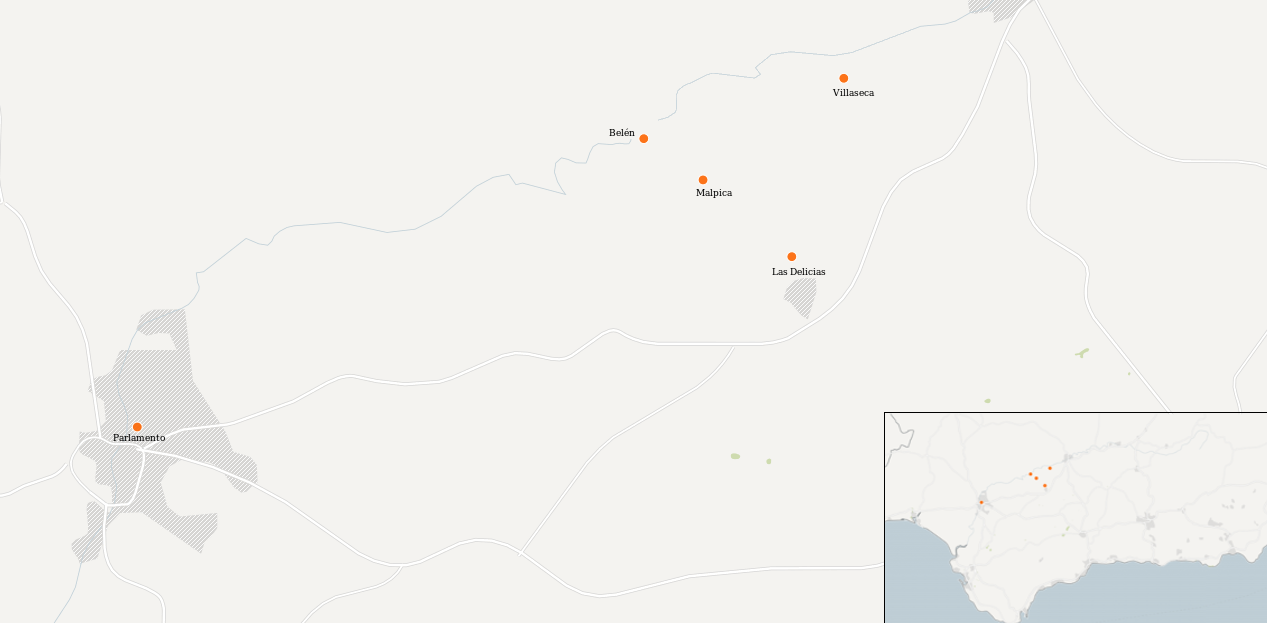
\includegraphics[width=0.7\linewidth]{images/fig1.png} &
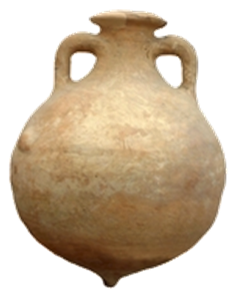
\includegraphics[width=0.2\linewidth]{images/amphorae.png} \\
(a) & (b)
\end{tabular}

\singlespace
\caption{a) More than 80 pottery workshops were distributed along the Guadalquivir river and its tributary the Genil. Red circles belong to the workshops analyzed. b) The entire sample is composed of Dressel 20 amphorae}
\label{fig:betica}
\end{figure}


 \end{block}
\end{column} % End of the first column

%BEGIN THE SECOND COLUMN-------------------------------------------------
\begin{column}{\twocolwid}


\begin{block}{Empirical Analysis}

\begin{columns}[t,totalwidth=\twocolwid]
\begin{column}{\onecolwid} %first subcolumn left


{\textbf{Methods}} 
\justify

Principal Component Analysis (PCA) allowed us to capture most of the variance of the 8 measurements into 2 variables. 


\end{column}

\begin{column}{\sepwid}\end{column} % Empty spacer column

\begin{column}{\onecolwid} %first subcolumn right

{\textbf{Results}}\\
\justify
The patterns observed in the first 2 Principal Components suggests that amphorae from closer workshops tend to be more similar (see Figure~\ref{fig:pca}). In particular, the three closest workshops show variation on PC1 (i.e. Bel\'en, Delicias and Malpica) while Parlamento displays a distinctive pattern than the rest of workshops on PC2 values.


\end{column}
 % End of the second column
\end{columns}

\begin{columns}[t,totalwidth=\twocolwid]


\begin{column}{\twocolwid} %first subcolumn left
\begin{figure}
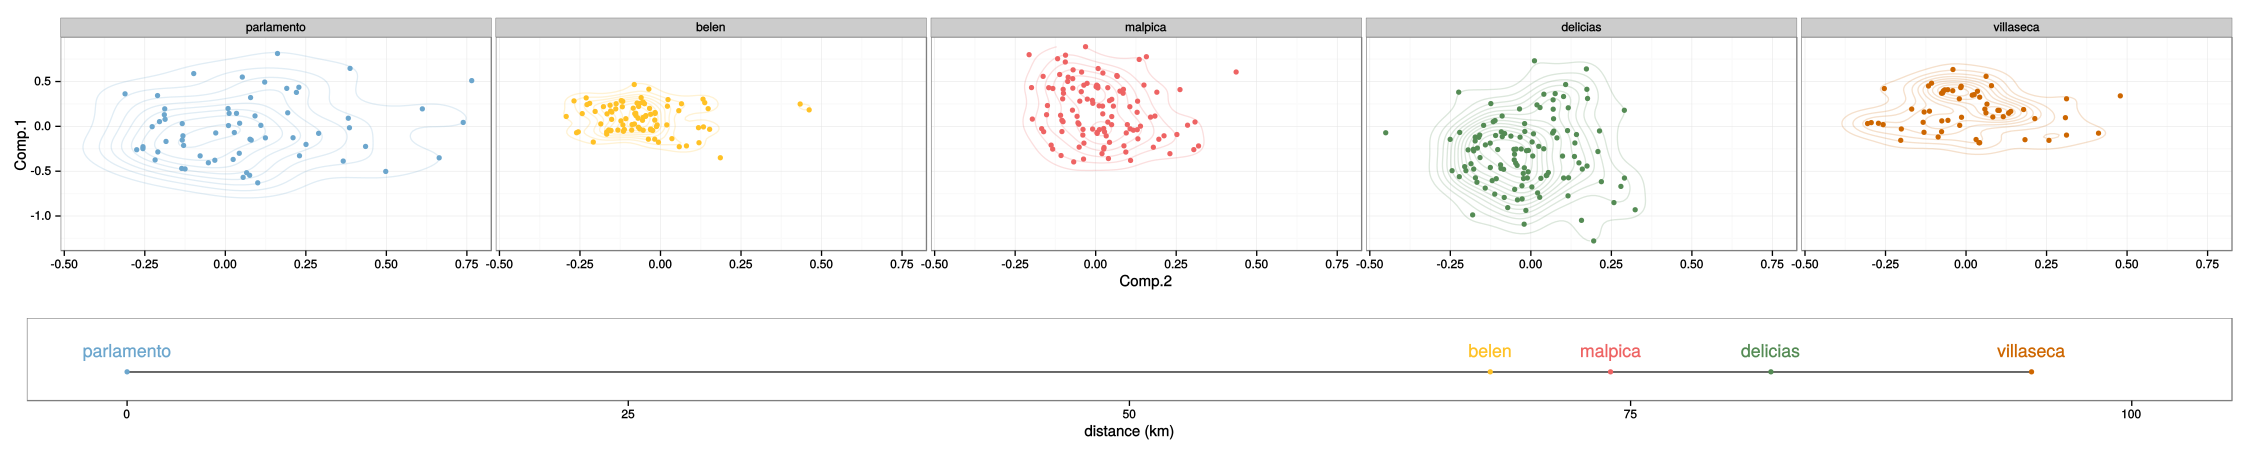
\includegraphics[width=0.6\linewidth]{images/fig2.png}
\singlespace
\caption{First and Second Principal Components for amphorae measured from the 4 analysed workshops}
\label{fig:pca}
\end{figure}
\end{column}
\end{columns}
\end{block}
\vspace{-1cm}
\begin{block}{Theoretical Exploration}

\begin{columns}[t,totalwidth=\twocolwid]

\begin{column}{1.025\onecolwid} %first subcolumn left
%on the left
{\textbf{Model }}
\justify
The observed pattern was further explored with a model based on classical random drift~\cite{bentley2004randomdriftandculturechange}. This approach allow us to test the impact of horizontal vs vertical transmission (HT vs VT) on the variation in production between workshops.  
We define a set $Pop$ of $N$ workshops sharing the same initial production techniques $P^{0}$ and positioned along a line at increasing distances (all workshops are positioned along the same river course).
Each workshop produce amphorae and change their production techniques by 1) modifying their own techniques or 2) copying one from another workshop.

The algorithm is defined as following:   


\begin{center}
    \fbox{

	\centering
	\begin{minipage}{.9\textwidth}
	%\begin{algorithm}[H]
	    \begin{algorithmic}
		\footnotesize
		\State INITIALIZATION:
		\For{$i \in Pop$}
		\State $P^{i} = P^{0}$
		\EndFor
		\State SIMULATION:
		\Loop{$~step \in TimeSteps$}
		\For{$i \in Pop$}
		\State $AmphoraProduction(P^{i})$
		\If{$ (step \mod 100) = 0$}	
		\State $P^{i}=Innovation(P^{i})$ \Comment{Vertical Transmission}
		\State $P^{i}=RandomCopy(Pop)$	\Comment{Horizontal Transmission}
		\EndIf
		\EndFor
		\EndLoop
	    \end{algorithmic}
	    %\caption{Model }
	    %\label{alg:mod}
	    %\line(1,0){\textwidth}
	%\end{algorithm}
	\end{minipage}

    }
\end{center}
\end{column}

\begin{column}{1.025\onecolwid} %first subcolumn right
{\textbf{Experiment \& Result}}\\
\justify
To test the impact of the distance we bias the random copy toward the closest neighbour. We define $P(T_{AB})$ the probability that $WS_A$ copy $WS_B$ as $\frac{1}{f(d)}$, where $d$ is the distance between $A$ and $B$. Three level of bias are tested. For each level we run $100$ simulations with 4 workshops. Amphorae are describe by on trait and we look how this trait varies between each workshop at the end of the simulation.

Figure~\ref{fig:resmod} shows that variation in production is high only if there is no HT or if the transfer is strongly biased toward the closest neighbour.
    \begin{figure}[h!]
	\begin{tabular}{cc}
	    \centering
	    External Diameter & Protruring Rim\\
	    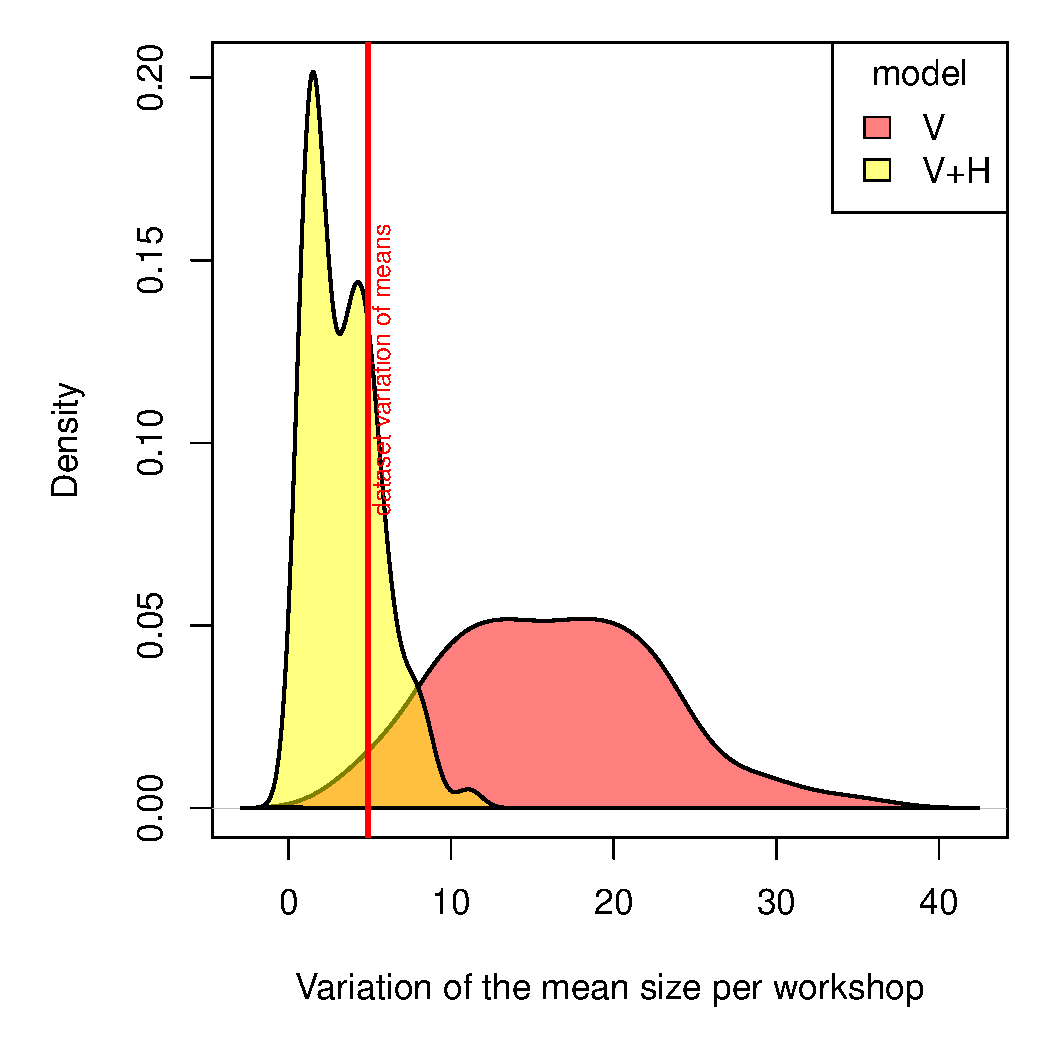
\includegraphics[width=0.4\linewidth]{images/ED_densities.pdf}&
	    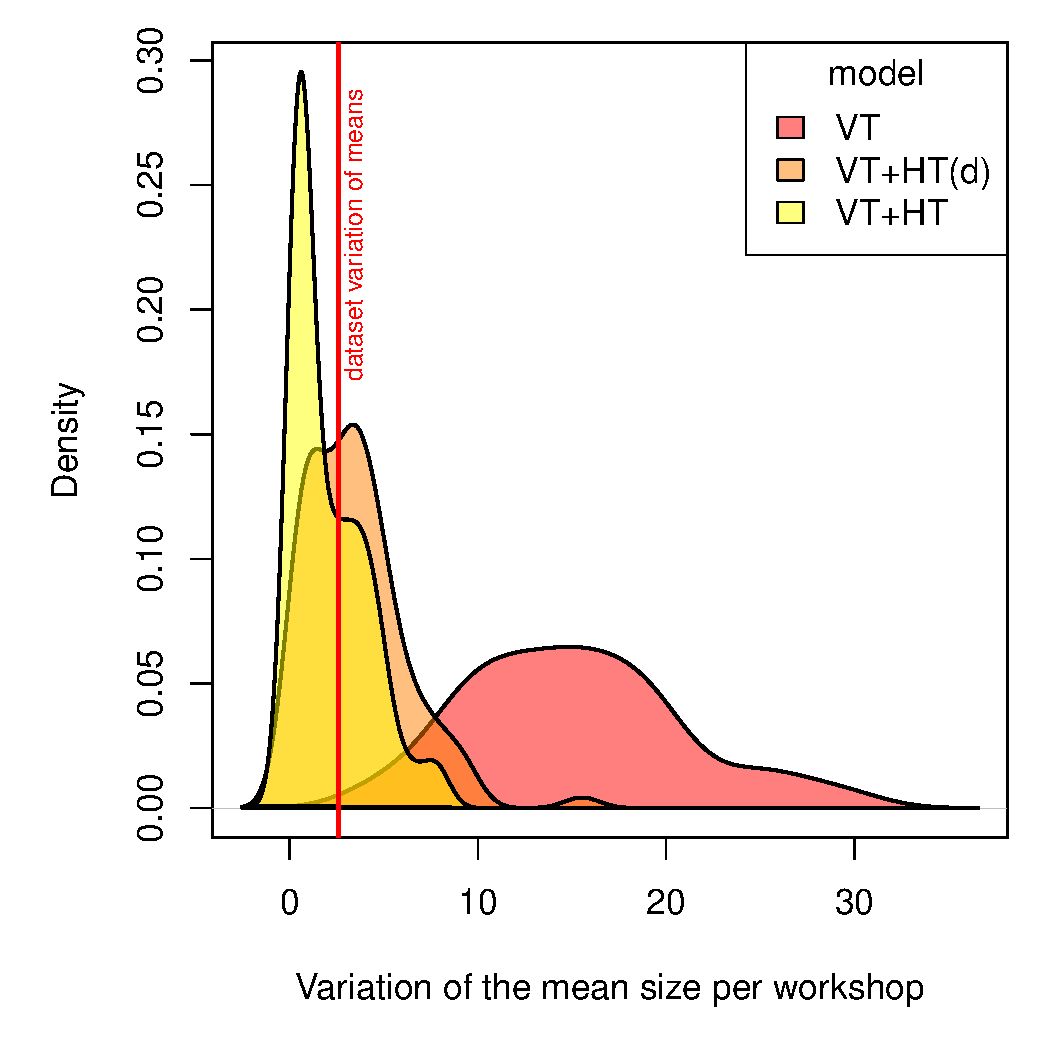
\includegraphics[width=0.4\linewidth]{images/PR_densities.pdf}\\
	\end{tabular}
\singlespace
\vspace{-.8cm}
\caption{Inter-workshop variation of the mean of the trait after $10\,000$ timestep in setup where the horizontal transfer probability varies (100 simulations per condition). The red line correspond to the variation measured on the real data}
	\label{fig:resmod}
    \end{figure}
\vspace{-1cm}
\end{column}
\end{columns}

\end{block}
\end{column}
% End of the second column

%BEGIN LAST COLUMN----------------------------------------------------

%\begin{column}{\sepwid}\end{column} % Empty spacer column

\begin{column}{\onecolwid} % The third column

\begin{block}{Discussion}
\justify

Empirical studies have identified variation on the making techniques processes among pottery workshops. We observe that this variability is affected by the distance: the analysed morphometric traits show that the similarity between amphorae decrease with the spatial distance between the workshops they were produced.

The combination of this empirical analysis with the theoretical model suggests that horizontal transmission could not be the main cultural process in the workshops. Vertical transmission seems to be the most probable mechanism. This can be interpreted by the fact that pottery techniques were learned from master to disciple and that disciples remained in the workshop where they were trained.
 
%\xavi{This sentence is repeating the information of the previous paragraph}.

\end{block}

\begin{block}{References}
\small

\begin{thebibliography}{50}


\bibitem[1]{lycett}\textsc{Lycett, S.J (2015)}
\textit{Cultural evolutionary approaches to artifact variation over time and space: basis, progress, and prospects}, Journal of Archaeological Science, 56, 21-31.

\bibitem[2]{bjo}\textsc{Bj\"{o}rklund, M., Bergek, S., Ranta, E., \& Kaitala, V. (2010)}
\textit{The effect of local population dynamics on patterns of isolation by distance}, Ecological Informatics, 5(3), 167-172.

\bibitem[3]{bentley2004randomdriftandculturechange}\textsc{Bentley, R., Hahn, M., Shennan, S. (2004)}
\textit{Random drift and culture change}, Proceedings of the Royal Society of London. Series B: Biological Sciences, 271(1547), 1443--1450.


\end{thebibliography}
%	\scriptsize
%	\renewcommand{\refname}{\vspace{-0.5em}}
%	//\bibliographystyle{abbrv}
%	\bibliography{biblio}

\end{block}

%----------------------------------------------------------------------------------------
%	ACKNOWLEDGEMENTS
%----------------------------------------------------------------------------------------

\setbeamercolor{block title}{fg=dblue,bg=white} % Change the block title color

\begin{block}{Acknowledgements}

\small{\rmfamily{The Funding for this work was provided by the ERC Advanced Grant EPNet (340828).}}

\end{block}

%----------------------------------------------------------------------------------------
%	CONTACT INFORMATION
%----------------------------------------------------------------------------------------

\setbeamercolor{block alerted title}{fg=white,bg=dblue!70} % Change the alert block title colors
\setbeamercolor{block alerted body}{fg=black,bg=white} % Change the alert block body colors


\begin{center}
\begin{tabular}{ccc}

\includegraphics[width=0.52\linewidth]{images/epnet.png} & \hfill & 
\includegraphics[width=0.5\linewidth]{images/erc.png}
\end{tabular}
\end{center}

%----------------------------------------------------------------------------------------

\end{column} % End of the third column

\end{columns} % End of all the columns in the poster

\end{frame} % End of the enclosing frame

\end{document}
